% Options for packages loaded elsewhere
\PassOptionsToPackage{unicode}{hyperref}
\PassOptionsToPackage{hyphens}{url}
%
\documentclass[
]{article}
\usepackage{amsmath,amssymb}
\usepackage{lmodern}
\usepackage{iftex}
\ifPDFTeX
  \usepackage[T1]{fontenc}
  \usepackage[utf8]{inputenc}
  \usepackage{textcomp} % provide euro and other symbols
\else % if luatex or xetex
  \usepackage{unicode-math}
  \defaultfontfeatures{Scale=MatchLowercase}
  \defaultfontfeatures[\rmfamily]{Ligatures=TeX,Scale=1}
\fi
% Use upquote if available, for straight quotes in verbatim environments
\IfFileExists{upquote.sty}{\usepackage{upquote}}{}
\IfFileExists{microtype.sty}{% use microtype if available
  \usepackage[]{microtype}
  \UseMicrotypeSet[protrusion]{basicmath} % disable protrusion for tt fonts
}{}
\makeatletter
\@ifundefined{KOMAClassName}{% if non-KOMA class
  \IfFileExists{parskip.sty}{%
    \usepackage{parskip}
  }{% else
    \setlength{\parindent}{0pt}
    \setlength{\parskip}{6pt plus 2pt minus 1pt}}
}{% if KOMA class
  \KOMAoptions{parskip=half}}
\makeatother
\usepackage{xcolor}
\usepackage[margin=1in]{geometry}
\usepackage{color}
\usepackage{fancyvrb}
\newcommand{\VerbBar}{|}
\newcommand{\VERB}{\Verb[commandchars=\\\{\}]}
\DefineVerbatimEnvironment{Highlighting}{Verbatim}{commandchars=\\\{\}}
% Add ',fontsize=\small' for more characters per line
\usepackage{framed}
\definecolor{shadecolor}{RGB}{248,248,248}
\newenvironment{Shaded}{\begin{snugshade}}{\end{snugshade}}
\newcommand{\AlertTok}[1]{\textcolor[rgb]{0.94,0.16,0.16}{#1}}
\newcommand{\AnnotationTok}[1]{\textcolor[rgb]{0.56,0.35,0.01}{\textbf{\textit{#1}}}}
\newcommand{\AttributeTok}[1]{\textcolor[rgb]{0.77,0.63,0.00}{#1}}
\newcommand{\BaseNTok}[1]{\textcolor[rgb]{0.00,0.00,0.81}{#1}}
\newcommand{\BuiltInTok}[1]{#1}
\newcommand{\CharTok}[1]{\textcolor[rgb]{0.31,0.60,0.02}{#1}}
\newcommand{\CommentTok}[1]{\textcolor[rgb]{0.56,0.35,0.01}{\textit{#1}}}
\newcommand{\CommentVarTok}[1]{\textcolor[rgb]{0.56,0.35,0.01}{\textbf{\textit{#1}}}}
\newcommand{\ConstantTok}[1]{\textcolor[rgb]{0.00,0.00,0.00}{#1}}
\newcommand{\ControlFlowTok}[1]{\textcolor[rgb]{0.13,0.29,0.53}{\textbf{#1}}}
\newcommand{\DataTypeTok}[1]{\textcolor[rgb]{0.13,0.29,0.53}{#1}}
\newcommand{\DecValTok}[1]{\textcolor[rgb]{0.00,0.00,0.81}{#1}}
\newcommand{\DocumentationTok}[1]{\textcolor[rgb]{0.56,0.35,0.01}{\textbf{\textit{#1}}}}
\newcommand{\ErrorTok}[1]{\textcolor[rgb]{0.64,0.00,0.00}{\textbf{#1}}}
\newcommand{\ExtensionTok}[1]{#1}
\newcommand{\FloatTok}[1]{\textcolor[rgb]{0.00,0.00,0.81}{#1}}
\newcommand{\FunctionTok}[1]{\textcolor[rgb]{0.00,0.00,0.00}{#1}}
\newcommand{\ImportTok}[1]{#1}
\newcommand{\InformationTok}[1]{\textcolor[rgb]{0.56,0.35,0.01}{\textbf{\textit{#1}}}}
\newcommand{\KeywordTok}[1]{\textcolor[rgb]{0.13,0.29,0.53}{\textbf{#1}}}
\newcommand{\NormalTok}[1]{#1}
\newcommand{\OperatorTok}[1]{\textcolor[rgb]{0.81,0.36,0.00}{\textbf{#1}}}
\newcommand{\OtherTok}[1]{\textcolor[rgb]{0.56,0.35,0.01}{#1}}
\newcommand{\PreprocessorTok}[1]{\textcolor[rgb]{0.56,0.35,0.01}{\textit{#1}}}
\newcommand{\RegionMarkerTok}[1]{#1}
\newcommand{\SpecialCharTok}[1]{\textcolor[rgb]{0.00,0.00,0.00}{#1}}
\newcommand{\SpecialStringTok}[1]{\textcolor[rgb]{0.31,0.60,0.02}{#1}}
\newcommand{\StringTok}[1]{\textcolor[rgb]{0.31,0.60,0.02}{#1}}
\newcommand{\VariableTok}[1]{\textcolor[rgb]{0.00,0.00,0.00}{#1}}
\newcommand{\VerbatimStringTok}[1]{\textcolor[rgb]{0.31,0.60,0.02}{#1}}
\newcommand{\WarningTok}[1]{\textcolor[rgb]{0.56,0.35,0.01}{\textbf{\textit{#1}}}}
\usepackage{graphicx}
\makeatletter
\def\maxwidth{\ifdim\Gin@nat@width>\linewidth\linewidth\else\Gin@nat@width\fi}
\def\maxheight{\ifdim\Gin@nat@height>\textheight\textheight\else\Gin@nat@height\fi}
\makeatother
% Scale images if necessary, so that they will not overflow the page
% margins by default, and it is still possible to overwrite the defaults
% using explicit options in \includegraphics[width, height, ...]{}
\setkeys{Gin}{width=\maxwidth,height=\maxheight,keepaspectratio}
% Set default figure placement to htbp
\makeatletter
\def\fps@figure{htbp}
\makeatother
\setlength{\emergencystretch}{3em} % prevent overfull lines
\providecommand{\tightlist}{%
  \setlength{\itemsep}{0pt}\setlength{\parskip}{0pt}}
\setcounter{secnumdepth}{-\maxdimen} % remove section numbering
\ifLuaTeX
  \usepackage{selnolig}  % disable illegal ligatures
\fi
\IfFileExists{bookmark.sty}{\usepackage{bookmark}}{\usepackage{hyperref}}
\IfFileExists{xurl.sty}{\usepackage{xurl}}{} % add URL line breaks if available
\urlstyle{same} % disable monospaced font for URLs
\hypersetup{
  hidelinks,
  pdfcreator={LaTeX via pandoc}}

\author{}
\date{\vspace{-2.5em}}

\begin{document}

{
\setcounter{tocdepth}{2}
\tableofcontents
}
\hypertarget{homework-5-trial-and-error}{%
\section{Homework 5: Trial and Error}\label{homework-5-trial-and-error}}

\hypertarget{buxf9i-khuxe1nh-duy---20001898}{%
\subsection{Bùi Khánh Duy -
20001898}\label{buxf9i-khuxe1nh-duy---20001898}}

\hypertarget{i.-luxed-thuyux1ebft-phux1b0ux1a1ng-phuxe1p}{%
\section{I. Lí thuyết phương
pháp}\label{i.-luxed-thuyux1ebft-phux1b0ux1a1ng-phuxe1p}}

Trình bày (ngắn gọn) ý tưởng và lược đồ tổng quát của 1 trong 3 phương
pháp:

\begin{itemize}
\tightlist
\item
  Vét cạn (Brute Force/Exhaustive);
\item
  Quay lui (Backtracking);
\item
  Nhánh cận (Branch and Bound).
\end{itemize}

\hypertarget{vuxe9t-cux1ea1n-brute-forceexhaustive}{%
\subsection{1. Vét cạn (Brute
Force/Exhaustive):}\label{vuxe9t-cux1ea1n-brute-forceexhaustive}}

Ý tưởng: Vét cạn là phương pháp duyệt tất cả các trường hợp có thể xảy
ra để tìm kiếm giải pháp cho bài toán. Phương pháp này thường được sử
dụng trong các bài toán có số lượng dữ liệu nhỏ và không yêu cầu tính
toán phức tạp.

Lược đồ tổng quát:

\begin{enumerate}
\def\labelenumi{\arabic{enumi}.}
\tightlist
\item
  Khởi tạo giá trị ban đầu.
\item
  Duyệt tất cả các trường hợp có thể xảy ra bằng vòng lặp hoặc đệ quy.
\item
  Kiểm tra điều kiện để xác định giải pháp.
\item
  Nếu tìm thấy giải pháp, trả về kết quả và kết thúc thuật toán.
\item
  Nếu không tìm thấy giải pháp, quay lại bước 2 và tiếp tục duyệt các
  trường hợp khác.
\end{enumerate}

\hypertarget{quay-lui-backtracking}{%
\subsection{2. Quay lui (Backtracking):}\label{quay-lui-backtracking}}

Ý tưởng: Quay lui là phương pháp tìm kiếm giải pháp cho các bài toán kết
hợp với việc lựa chọn và loại bỏ các phương án. Phương pháp này thường
được sử dụng trong các bài toán tìm kiếm đường đi, sắp xếp, chia nhỏ và
thống kê.

Lược đồ tổng quát:

\begin{enumerate}
\def\labelenumi{\arabic{enumi}.}
\tightlist
\item
  Khởi tạo giá trị ban đầu.
\item
  Lựa chọn một phương án và thực hiện nó.
\item
  Kiểm tra điều kiện để xác định giải pháp.
\item
  Nếu tìm thấy giải pháp, trả về kết quả và kết thúc thuật toán.
\item
  Nếu không tìm thấy giải pháp, quay lại bước 2, loại bỏ phương án vừa
  chọn và thử phương án khác.
\end{enumerate}

\hypertarget{nhuxe1nh-cux1eadn-branch-and-bound}{%
\subsection{3. Nhánh cận (Branch and
Bound):}\label{nhuxe1nh-cux1eadn-branch-and-bound}}

Ý tưởng: Nhánh cận là phương pháp tìm kiếm giải pháp cho các bài toán
tối ưu. Phương pháp này tìm kiếm các giải pháp tiềm năng và loại bỏ
những giải pháp không cần thiết trước khi tìm kiếm các giải pháp khác.

Lược đồ tổng quát:

\begin{enumerate}
\def\labelenumi{\arabic{enumi}.}
\tightlist
\item
  Khởi tạo giá trị ban đầu.
\item
  Tìm kiếm các giải pháp tiềm năng và tính toán giá trị của chúng.
\item
  Loại bỏ giải pháp không cần thiết và chỉ giữ lại những giải pháp tiềm
  năng tốt nhất.
\item
  Tạo các nhánh mới cho các giải pháp tiềm năng tốt nhất và tiếp tục tìm
  kiếm giải pháp trong các nhánh này.
\item
  Kiểm tra điều kiện để xác định giải pháp tối ưu.
\item
  Nếu tìm thấy giải pháp tối ưu, trả về kết quả và kết thúc thuật toán.
\item
  Nếu không tìm thấy giải pháp tối ưu, quay lại bước 3 và tiếp tục loại
  bỏ giải pháp không cần thiết.
\end{enumerate}

\hypertarget{ii.-lux1eadp-truxecnh}{%
\section{II. Lập trình}\label{ii.-lux1eadp-truxecnh}}

\hypertarget{khux1edbp-xuxe2u}{%
\subsection{Khớp xâu}\label{khux1edbp-xuxe2u}}

Sử dụng thuật toán \textbf{Rabin-Karp}

\hypertarget{buxe0i-touxe1n}{%
\subsubsection{Bài toán}\label{buxe0i-touxe1n}}

Cho 2 xâu: xâu cần tìm \(s\) và đoạn văn bản \(t\). Kiểm tra xem \(s\)
có xuất hiện trong \(t\) hay không? Nếu có, liệt kê tất cả các vị trí
của nó với độ phức tạp thời gian \(O(|s| + |t|)\)

\hypertarget{uxfd-tux1b0ux1edfng-cux1ee7a-thuux1eadt-touxe1n}{%
\subsubsection{Ý tưởng của thuật
toán:}\label{uxfd-tux1b0ux1edfng-cux1ee7a-thuux1eadt-touxe1n}}

Sử dụng hàm băm (hash) cho xâu \(s\). Tính giá trị của hàm băm với tất
cả các tiền tố của xâu \(t\). Sau đó có thể kiểu tra \(s\) với các xâu
con có độ dài \(|s|\) trong thời gian \(O(1)\), tổng cộng sẽ mất
\(O(|t|)\).

Tổng độ phức tạp thời gian là \(O(|t|+|s|)\).

\hypertarget{code-c}{%
\subsubsection{Code (C++)}\label{code-c}}

\begin{Shaded}
\begin{Highlighting}[]
\PreprocessorTok{\#include }\ImportTok{\textless{}bits/stdc++.h\textgreater{}}
\KeywordTok{using} \KeywordTok{namespace}\NormalTok{ std}\OperatorTok{;}

\NormalTok{vector}\OperatorTok{\textless{}}\DataTypeTok{int}\OperatorTok{\textgreater{}}\NormalTok{ rabin\_karp}\OperatorTok{(}\NormalTok{string }\AttributeTok{const}\OperatorTok{\&}\NormalTok{ s}\OperatorTok{,}\NormalTok{ string }\AttributeTok{const}\OperatorTok{\&}\NormalTok{ t}\OperatorTok{)} \OperatorTok{\{}
    \AttributeTok{const} \DataTypeTok{int}\NormalTok{ p }\OperatorTok{=} \DecValTok{31}\OperatorTok{;} 
    \AttributeTok{const} \DataTypeTok{int}\NormalTok{ m }\OperatorTok{=} \FloatTok{1e9} \OperatorTok{+} \DecValTok{9}\OperatorTok{;}
    \DataTypeTok{int}\NormalTok{ S }\OperatorTok{=}\NormalTok{ s}\OperatorTok{.}\NormalTok{size}\OperatorTok{(),}\NormalTok{ T }\OperatorTok{=}\NormalTok{ t}\OperatorTok{.}\NormalTok{size}\OperatorTok{();}

\NormalTok{    vector}\OperatorTok{\textless{}}\DataTypeTok{long} \DataTypeTok{long}\OperatorTok{\textgreater{}}\NormalTok{ p\_pow}\OperatorTok{(}\NormalTok{max}\OperatorTok{(}\NormalTok{S}\OperatorTok{,}\NormalTok{ T}\OperatorTok{));} 
\NormalTok{    p\_pow}\OperatorTok{[}\DecValTok{0}\OperatorTok{]} \OperatorTok{=} \DecValTok{1}\OperatorTok{;} 
    \ControlFlowTok{for} \OperatorTok{(}\DataTypeTok{int}\NormalTok{ i }\OperatorTok{=} \DecValTok{1}\OperatorTok{;}\NormalTok{ i }\OperatorTok{\textless{}} \OperatorTok{(}\DataTypeTok{int}\OperatorTok{)}\NormalTok{p\_pow}\OperatorTok{.}\NormalTok{size}\OperatorTok{();}\NormalTok{ i}\OperatorTok{++)} 
\NormalTok{        p\_pow}\OperatorTok{[}\NormalTok{i}\OperatorTok{]} \OperatorTok{=} \OperatorTok{(}\NormalTok{p\_pow}\OperatorTok{[}\NormalTok{i}\OperatorTok{{-}}\DecValTok{1}\OperatorTok{]} \OperatorTok{*}\NormalTok{ p}\OperatorTok{)} \OperatorTok{\%}\NormalTok{ m}\OperatorTok{;}

\NormalTok{    vector}\OperatorTok{\textless{}}\DataTypeTok{long} \DataTypeTok{long}\OperatorTok{\textgreater{}}\NormalTok{ hashing}\OperatorTok{(}\NormalTok{T }\OperatorTok{+} \DecValTok{1}\OperatorTok{,} \DecValTok{0}\OperatorTok{);} 
    \ControlFlowTok{for} \OperatorTok{(}\DataTypeTok{int}\NormalTok{ i }\OperatorTok{=} \DecValTok{0}\OperatorTok{;}\NormalTok{ i }\OperatorTok{\textless{}}\NormalTok{ T}\OperatorTok{;}\NormalTok{ i}\OperatorTok{++)}
\NormalTok{        hashing}\OperatorTok{[}\NormalTok{i}\OperatorTok{+}\DecValTok{1}\OperatorTok{]} \OperatorTok{=} \OperatorTok{(}\NormalTok{hashing}\OperatorTok{[}\NormalTok{i}\OperatorTok{]} \OperatorTok{+} \OperatorTok{(}\NormalTok{t}\OperatorTok{[}\NormalTok{i}\OperatorTok{]} \OperatorTok{{-}} \CharTok{\textquotesingle{}a\textquotesingle{}} \OperatorTok{+} \DecValTok{1}\OperatorTok{)} \OperatorTok{*}\NormalTok{ p\_pow}\OperatorTok{[}\NormalTok{i}\OperatorTok{])} \OperatorTok{\%}\NormalTok{ m}\OperatorTok{;} 
    \DataTypeTok{long} \DataTypeTok{long}\NormalTok{ h\_s }\OperatorTok{=} \DecValTok{0}\OperatorTok{;} 
    \ControlFlowTok{for} \OperatorTok{(}\DataTypeTok{int}\NormalTok{ i }\OperatorTok{=} \DecValTok{0}\OperatorTok{;}\NormalTok{ i }\OperatorTok{\textless{}}\NormalTok{ S}\OperatorTok{;}\NormalTok{ i}\OperatorTok{++)} 
\NormalTok{        h\_s }\OperatorTok{=} \OperatorTok{(}\NormalTok{h\_s }\OperatorTok{+} \OperatorTok{(}\NormalTok{s}\OperatorTok{[}\NormalTok{i}\OperatorTok{]} \OperatorTok{{-}} \CharTok{\textquotesingle{}a\textquotesingle{}} \OperatorTok{+} \DecValTok{1}\OperatorTok{)} \OperatorTok{*}\NormalTok{ p\_pow}\OperatorTok{[}\NormalTok{i}\OperatorTok{])} \OperatorTok{\%}\NormalTok{ m}\OperatorTok{;} 

\NormalTok{    vector}\OperatorTok{\textless{}}\DataTypeTok{int}\OperatorTok{\textgreater{}}\NormalTok{ occurrences}\OperatorTok{;}
    \ControlFlowTok{for} \OperatorTok{(}\DataTypeTok{int}\NormalTok{ i }\OperatorTok{=} \DecValTok{0}\OperatorTok{;}\NormalTok{ i }\OperatorTok{+}\NormalTok{ S }\OperatorTok{{-}} \DecValTok{1} \OperatorTok{\textless{}}\NormalTok{ T}\OperatorTok{;}\NormalTok{ i}\OperatorTok{++)} \OperatorTok{\{} 
        \DataTypeTok{long} \DataTypeTok{long}\NormalTok{ cur\_h }\OperatorTok{=} \OperatorTok{(}\NormalTok{hashing}\OperatorTok{[}\NormalTok{i}\OperatorTok{+}\NormalTok{S}\OperatorTok{]} \OperatorTok{+}\NormalTok{ m }\OperatorTok{{-}}\NormalTok{ hashing}\OperatorTok{[}\NormalTok{i}\OperatorTok{])} \OperatorTok{\%}\NormalTok{ m}\OperatorTok{;} 
        \ControlFlowTok{if} \OperatorTok{(}\NormalTok{cur\_h }\OperatorTok{==}\NormalTok{ h\_s }\OperatorTok{*}\NormalTok{ p\_pow}\OperatorTok{[}\NormalTok{i}\OperatorTok{]} \OperatorTok{\%}\NormalTok{ m}\OperatorTok{)}
\NormalTok{            occurrences}\OperatorTok{.}\NormalTok{push\_back}\OperatorTok{(}\NormalTok{i}\OperatorTok{);}
    \OperatorTok{\}}
    \ControlFlowTok{return}\NormalTok{ occurrences}\OperatorTok{;}
\OperatorTok{\}}
\end{Highlighting}
\end{Shaded}

\hypertarget{duxe3y-nhux1ecb-phuxe2n}{%
\subsection{Dãy nhị phân}\label{duxe3y-nhux1ecb-phuxe2n}}

Liệt kê các dãy nhị phân có độ dài n.

Có 2 cách code:

\hypertarget{c1-ux111ux1ec7-quy}{%
\subsubsection{C1: Đệ quy}\label{c1-ux111ux1ec7-quy}}

\begin{Shaded}
\begin{Highlighting}[]
\KeywordTok{def}\NormalTok{ generateBinary(n, current):}
    \ControlFlowTok{if}\NormalTok{ n }\OperatorTok{==} \DecValTok{0}\NormalTok{:}
\NormalTok{        result.append(current)}
        \ControlFlowTok{return}
    \ControlFlowTok{for}\NormalTok{ i }\KeywordTok{in} \BuiltInTok{range}\NormalTok{(}\DecValTok{2}\NormalTok{):}
\NormalTok{        generateBinary(n}\OperatorTok{{-}}\DecValTok{1}\NormalTok{, current }\OperatorTok{+} \BuiltInTok{str}\NormalTok{(i))}

\KeywordTok{def}\NormalTok{ binary\_list(n):}
\NormalTok{        generateBinary(n, }\StringTok{""}\NormalTok{)}
        \ControlFlowTok{return}\NormalTok{ result}
\NormalTok{result }\OperatorTok{=}\NormalTok{ []}
\NormalTok{binary\_list(}\DecValTok{5}\NormalTok{)}\OperatorTok{;}
\BuiltInTok{print}\NormalTok{(result)}
\end{Highlighting}
\end{Shaded}

Kết quả

\begin{Shaded}
\begin{Highlighting}[]
\NormalTok{[}\StringTok{\textquotesingle{}00000\textquotesingle{}}\NormalTok{, }\StringTok{\textquotesingle{}00001\textquotesingle{}}\NormalTok{, }\StringTok{\textquotesingle{}00010\textquotesingle{}}\NormalTok{, }\StringTok{\textquotesingle{}00011\textquotesingle{}}\NormalTok{, }\StringTok{\textquotesingle{}00100\textquotesingle{}}\NormalTok{, }\StringTok{\textquotesingle{}00101\textquotesingle{}}\NormalTok{, }\StringTok{\textquotesingle{}00110\textquotesingle{}}\NormalTok{, }\StringTok{\textquotesingle{}00111\textquotesingle{}}\NormalTok{, }\StringTok{\textquotesingle{}01000\textquotesingle{}}\NormalTok{, }\StringTok{\textquotesingle{}01001\textquotesingle{}}\NormalTok{, }\StringTok{\textquotesingle{}01010\textquotesingle{}}\NormalTok{, }\StringTok{\textquotesingle{}01011\textquotesingle{}}\NormalTok{, }\StringTok{\textquotesingle{}01100\textquotesingle{}}\NormalTok{, }\StringTok{\textquotesingle{}01101\textquotesingle{}}\NormalTok{, }\StringTok{\textquotesingle{}01110\textquotesingle{}}\NormalTok{, }\StringTok{\textquotesingle{}01111\textquotesingle{}}\NormalTok{, }\StringTok{\textquotesingle{}10000\textquotesingle{}}\NormalTok{, }\StringTok{\textquotesingle{}10001\textquotesingle{}}\NormalTok{, }\StringTok{\textquotesingle{}10010\textquotesingle{}}\NormalTok{, }\StringTok{\textquotesingle{}10011\textquotesingle{}}\NormalTok{, }\StringTok{\textquotesingle{}10100\textquotesingle{}}\NormalTok{, }\StringTok{\textquotesingle{}10101\textquotesingle{}}\NormalTok{, }\StringTok{\textquotesingle{}10110\textquotesingle{}}\NormalTok{, }\StringTok{\textquotesingle{}10111\textquotesingle{}}\NormalTok{, }\StringTok{\textquotesingle{}11000\textquotesingle{}}\NormalTok{, }\StringTok{\textquotesingle{}11001\textquotesingle{}}\NormalTok{, }\StringTok{\textquotesingle{}11010\textquotesingle{}}\NormalTok{, }\StringTok{\textquotesingle{}11011\textquotesingle{}}\NormalTok{, }\StringTok{\textquotesingle{}11100\textquotesingle{}}\NormalTok{, }\StringTok{\textquotesingle{}11101\textquotesingle{}}\NormalTok{, }\StringTok{\textquotesingle{}11110\textquotesingle{}}\NormalTok{, }\StringTok{\textquotesingle{}11111\textquotesingle{}}\NormalTok{]}
\end{Highlighting}
\end{Shaded}

\hypertarget{c2-khux1eed-ux111ux1ec7-quy}{%
\subsubsection{C2: Khử đệ quy}\label{c2-khux1eed-ux111ux1ec7-quy}}

\begin{Shaded}
\begin{Highlighting}[]
\KeywordTok{def}\NormalTok{ binary\_list2(n):}
\NormalTok{    result }\OperatorTok{=}\NormalTok{ []}
    \ControlFlowTok{for}\NormalTok{ i }\KeywordTok{in} \BuiltInTok{range}\NormalTok{(}\DecValTok{1}\OperatorTok{\textless{}\textless{}}\NormalTok{n):}
\NormalTok{        result.append(}\BuiltInTok{bin}\NormalTok{(i)[}\DecValTok{2}\NormalTok{:].zfill(n))}
    \ControlFlowTok{return}\NormalTok{ result}
\BuiltInTok{print}\NormalTok{(binary\_list2(}\DecValTok{5}\NormalTok{))}
\end{Highlighting}
\end{Shaded}

\begin{Shaded}
\begin{Highlighting}[]
\NormalTok{[}\StringTok{\textquotesingle{}00000\textquotesingle{}}\NormalTok{, }\StringTok{\textquotesingle{}00001\textquotesingle{}}\NormalTok{, }\StringTok{\textquotesingle{}00010\textquotesingle{}}\NormalTok{, }\StringTok{\textquotesingle{}00011\textquotesingle{}}\NormalTok{, }\StringTok{\textquotesingle{}00100\textquotesingle{}}\NormalTok{, }\StringTok{\textquotesingle{}00101\textquotesingle{}}\NormalTok{, }\StringTok{\textquotesingle{}00110\textquotesingle{}}\NormalTok{, }\StringTok{\textquotesingle{}00111\textquotesingle{}}\NormalTok{, }\StringTok{\textquotesingle{}01000\textquotesingle{}}\NormalTok{, }\StringTok{\textquotesingle{}01001\textquotesingle{}}\NormalTok{, }\StringTok{\textquotesingle{}01010\textquotesingle{}}\NormalTok{, }\StringTok{\textquotesingle{}01011\textquotesingle{}}\NormalTok{, }\StringTok{\textquotesingle{}01100\textquotesingle{}}\NormalTok{, }\StringTok{\textquotesingle{}01101\textquotesingle{}}\NormalTok{, }\StringTok{\textquotesingle{}01110\textquotesingle{}}\NormalTok{, }\StringTok{\textquotesingle{}01111\textquotesingle{}}\NormalTok{, }\StringTok{\textquotesingle{}10000\textquotesingle{}}\NormalTok{, }\StringTok{\textquotesingle{}10001\textquotesingle{}}\NormalTok{, }\StringTok{\textquotesingle{}10010\textquotesingle{}}\NormalTok{, }\StringTok{\textquotesingle{}10011\textquotesingle{}}\NormalTok{, }\StringTok{\textquotesingle{}10100\textquotesingle{}}\NormalTok{, }\StringTok{\textquotesingle{}10101\textquotesingle{}}\NormalTok{, }\StringTok{\textquotesingle{}10110\textquotesingle{}}\NormalTok{, }\StringTok{\textquotesingle{}10111\textquotesingle{}}\NormalTok{, }\StringTok{\textquotesingle{}11000\textquotesingle{}}\NormalTok{, }\StringTok{\textquotesingle{}11001\textquotesingle{}}\NormalTok{, }\StringTok{\textquotesingle{}11010\textquotesingle{}}\NormalTok{, }\StringTok{\textquotesingle{}11011\textquotesingle{}}\NormalTok{, }\StringTok{\textquotesingle{}11100\textquotesingle{}}\NormalTok{, }\StringTok{\textquotesingle{}11101\textquotesingle{}}\NormalTok{, }\StringTok{\textquotesingle{}11110\textquotesingle{}}\NormalTok{, }\StringTok{\textquotesingle{}11111\textquotesingle{}}\NormalTok{]}
\end{Highlighting}
\end{Shaded}

Cả 2 đều có độ phức tạp thuật toán \(O(2^n)\)

\hypertarget{iii.-ux111ux1eb7t-buxe0i-touxe1n-thiux1ebft-kux1ebf-phuxe2n-tuxedch-vuxe0-triux1ec3n-khai-thuux1eadt-touxe1n}{%
\section{III. Đặt bài toán, thiết kế, phân tích và triển khai thuật
toán}\label{iii.-ux111ux1eb7t-buxe0i-touxe1n-thiux1ebft-kux1ebf-phuxe2n-tuxedch-vuxe0-triux1ec3n-khai-thuux1eadt-touxe1n}}

Lưu ý: Ở đây sẽ dùng ngôn ngữ \texttt{C++}

\hypertarget{buxe0i-touxe1n-1}{%
\subsection{Bài toán}\label{buxe0i-touxe1n-1}}

Hãy chỉ ra một cách đi của con mã để xuất phát từ một ô cờ \((x,y)\) nào
đó \((x,y=\overline{1...8})\) có thể đi qua tất cả các ô cờ, mỗi ô duy
nhất một lần.

\href{https://en.wikipedia.org/wiki/Knight\textquotesingle{}s_tour}{Knight\textquotesingle s
tour}

Tên tiếng anh: \textbf{Knight tour}

Tên tiếng việt: Mã đi tuần.

\begin{figure}
\centering
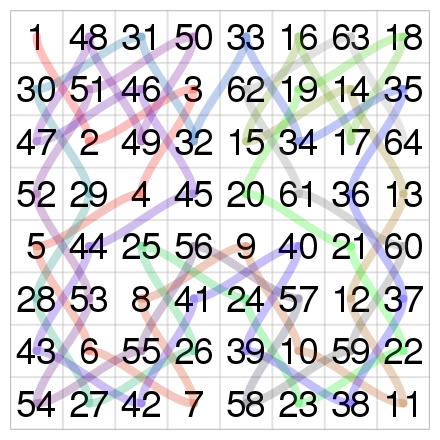
\includegraphics[width=3.125in,height=3.125in]{Homework 5 Trial and Error 3b646dc8160042df9d000a4baa7eeb4e/Untitled.png}
\caption{Một đáp án giải cho bài toán này (bàn cờ 8x8)}
\end{figure}

\hypertarget{muxf4-tux1ea3-buxe0i-touxe1n}{%
\subsubsection{Mô tả bài toán}\label{muxf4-tux1ea3-buxe0i-touxe1n}}

Cho bàn cờ \(N\times N\) với quân mã đặt ở 1 vị trí bất kì (để cho đơn
giản, quân mã được đặt ở vị trí \(1,1\)). Quân mã cần di chuyển trên bàn
cờ theo đúng luật, với mỗi ô được đi qua đúng 1 lần. In ra thứ tự của
các ô được đi qua.

\begin{Shaded}
\begin{Highlighting}[]
\NormalTok{Input : }
\NormalTok{N = 8}
\NormalTok{Output:}
\NormalTok{0  59  38  33  30  17   8  63}
\NormalTok{37  34  31  60   9  62  29  16}
\NormalTok{58   1  36  39  32  27  18   7}
\NormalTok{35  48  41  26  61  10  15  28}
\NormalTok{42  57   2  49  40  23   6  19}
\NormalTok{47  50  45  54  25  20  11  14}
\NormalTok{56  43  52   3  22  13  24   5}
\NormalTok{51  46  55  44  53   4  21  12}
\end{Highlighting}
\end{Shaded}

\hypertarget{phuxe2n-tuxedch}{%
\subsubsection{Phân tích}\label{phuxe2n-tuxedch}}

Quân mã ở đỉnh \((i, j)\) có thể di chuyển đến 8 đỉnh khác

\begin{figure}
\centering
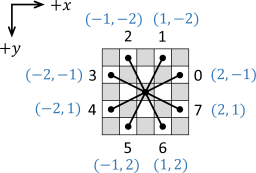
\includegraphics{Homework 5 Trial and Error 3b646dc8160042df9d000a4baa7eeb4e/Untitled 1.png}
\caption{Các hướng của quân mã}
\end{figure}

Từ đó ta có thể định nghĩa trước các cặp \((dx, dy)\) tương ứng với 8
hướng có thể đi

\begin{Shaded}
\begin{Highlighting}[]
\DataTypeTok{int}\NormalTok{ dx}\OperatorTok{[]} \OperatorTok{=} \OperatorTok{\{{-}}\DecValTok{2}\OperatorTok{,} \OperatorTok{{-}}\DecValTok{2}\OperatorTok{,} \OperatorTok{{-}}\DecValTok{1}\OperatorTok{,} \OperatorTok{{-}}\DecValTok{1}\OperatorTok{,} \DecValTok{1}\OperatorTok{,} \DecValTok{1}\OperatorTok{,} \DecValTok{2}\OperatorTok{,} \DecValTok{2}\OperatorTok{\};}
\DataTypeTok{int}\NormalTok{ dy}\OperatorTok{[]} \OperatorTok{=} \OperatorTok{\{{-}}\DecValTok{1}\OperatorTok{,} \DecValTok{1}\OperatorTok{,} \OperatorTok{{-}}\DecValTok{2}\OperatorTok{,} \DecValTok{2}\OperatorTok{,} \OperatorTok{{-}}\DecValTok{2}\OperatorTok{,} \DecValTok{2}\OperatorTok{,} \OperatorTok{{-}}\DecValTok{1}\OperatorTok{,} \DecValTok{1}\OperatorTok{\};}
\end{Highlighting}
\end{Shaded}

Các hướng giải quyết

\hypertarget{backtracking}{%
\subsubsection{Backtracking}\label{backtracking}}

Ý tưởng giải bằng phương pháp này khá đơn giản, có các bước như sau

\begin{enumerate}
\def\labelenumi{\arabic{enumi}.}
\tightlist
\item
  Thêm 1 đỉnh vào tập lời giải, đánh dấu lại đỉnh này đã đi qua và đi
  đến một trong 8 hướng còn lại
\item
  Nếu đỉnh hiện tại không đi đủ thành 1 vòng \textasciitilde{} nghiệm
  sai ⇒ quay lại để giải theo hướng khác, đồng thời cũng xoá các trạng
  thái của đường đi đang có.
\item
  Sau khi duyệt hết tất cả các trường hợp, nếu không có kết quả ⇒ In ra
  màn hình \texttt{Not\ found!}, ngược lại in ra ma trận có dạng như ở
  ví dụ
\end{enumerate}

\begin{Shaded}
\begin{Highlighting}[]
\PreprocessorTok{\#include}\ImportTok{\textless{}vector\textgreater{}}
\PreprocessorTok{\#include}\ImportTok{\textless{}utility\textgreater{}}
\PreprocessorTok{\#include}\ImportTok{\textless{}iostream\textgreater{}}
\KeywordTok{using} \KeywordTok{namespace}\NormalTok{ std}\OperatorTok{;}
\PreprocessorTok{\#define IOS }\NormalTok{ios}\OperatorTok{::}\NormalTok{sync\_with\_stdio}\OperatorTok{(}\DecValTok{0}\OperatorTok{);}\PreprocessorTok{ }\NormalTok{cin}\OperatorTok{.}\NormalTok{tie}\OperatorTok{(}\DecValTok{0}\OperatorTok{);}\PreprocessorTok{ }\NormalTok{cout}\OperatorTok{.}\NormalTok{tie}\OperatorTok{(}\DecValTok{0}\OperatorTok{);}

\DataTypeTok{int}\NormalTok{ N}\OperatorTok{;}
\DataTypeTok{int}\NormalTok{ dx}\OperatorTok{[]} \OperatorTok{=} \OperatorTok{\{{-}}\DecValTok{2}\OperatorTok{,} \OperatorTok{{-}}\DecValTok{2}\OperatorTok{,} \OperatorTok{{-}}\DecValTok{1}\OperatorTok{,} \OperatorTok{{-}}\DecValTok{1}\OperatorTok{,} \DecValTok{1}\OperatorTok{,} \DecValTok{1}\OperatorTok{,} \DecValTok{2}\OperatorTok{,} \DecValTok{2}\OperatorTok{\};}
\DataTypeTok{int}\NormalTok{ dy}\OperatorTok{[]} \OperatorTok{=} \OperatorTok{\{{-}}\DecValTok{1}\OperatorTok{,} \DecValTok{1}\OperatorTok{,} \OperatorTok{{-}}\DecValTok{2}\OperatorTok{,} \DecValTok{2}\OperatorTok{,} \OperatorTok{{-}}\DecValTok{2}\OperatorTok{,} \DecValTok{2}\OperatorTok{,} \OperatorTok{{-}}\DecValTok{1}\OperatorTok{,} \DecValTok{1}\OperatorTok{\};}

\NormalTok{pair}\OperatorTok{\textless{}}\DataTypeTok{int}\OperatorTok{,} \DataTypeTok{int}\OperatorTok{\textgreater{}} \KeywordTok{operator}\OperatorTok{+} \OperatorTok{(}\AttributeTok{const}\NormalTok{ pair}\OperatorTok{\textless{}}\DataTypeTok{int}\OperatorTok{,} \DataTypeTok{int}\OperatorTok{\textgreater{}\&}\NormalTok{ a}\OperatorTok{,} \AttributeTok{const}\NormalTok{ pair}\OperatorTok{\textless{}}\DataTypeTok{int}\OperatorTok{,} \DataTypeTok{int}\OperatorTok{\textgreater{}\&}\NormalTok{ b}\OperatorTok{)} \OperatorTok{\{}
    \ControlFlowTok{return} \OperatorTok{\{}\NormalTok{a}\OperatorTok{.}\NormalTok{first }\OperatorTok{+}\NormalTok{ b}\OperatorTok{.}\NormalTok{first}\OperatorTok{,}\NormalTok{ a}\OperatorTok{.}\NormalTok{second }\OperatorTok{+}\NormalTok{ b}\OperatorTok{.}\NormalTok{second}\OperatorTok{\};}
\OperatorTok{\}}
\DataTypeTok{bool} \KeywordTok{operator}\OperatorTok{==} \OperatorTok{(}\AttributeTok{const}\NormalTok{ pair}\OperatorTok{\textless{}}\DataTypeTok{int}\OperatorTok{,} \DataTypeTok{int}\OperatorTok{\textgreater{}\&}\NormalTok{ a}\OperatorTok{,} \AttributeTok{const}\NormalTok{ pair}\OperatorTok{\textless{}}\DataTypeTok{int}\OperatorTok{,} \DataTypeTok{int}\OperatorTok{\textgreater{}\&}\NormalTok{ b}\OperatorTok{)} \OperatorTok{\{}
    \ControlFlowTok{return}\NormalTok{ a}\OperatorTok{.}\NormalTok{first }\OperatorTok{==}\NormalTok{ b}\OperatorTok{.}\NormalTok{first }\OperatorTok{\&\&}\NormalTok{ a}\OperatorTok{.}\NormalTok{second }\OperatorTok{==}\NormalTok{ b}\OperatorTok{.}\NormalTok{second}\OperatorTok{;}
\OperatorTok{\}}
\NormalTok{vector}\OperatorTok{\textless{}}\NormalTok{pair}\OperatorTok{\textless{}}\DataTypeTok{int}\OperatorTok{,} \DataTypeTok{int}\OperatorTok{\textgreater{}\textgreater{}}\NormalTok{ path}\OperatorTok{,}\NormalTok{ ans}\OperatorTok{;}
\CommentTok{// vector\textless{}vector\textless{}pair\textless{}int, int\textgreater{}\textgreater{}\textgreater{} ans;}
\NormalTok{vector}\OperatorTok{\textless{}}\NormalTok{vector}\OperatorTok{\textless{}}\DataTypeTok{bool}\OperatorTok{\textgreater{}\textgreater{}}\NormalTok{ check}\OperatorTok{;}
\DataTypeTok{void}\NormalTok{ solve}\OperatorTok{();}
\DataTypeTok{void}\NormalTok{ out}\OperatorTok{()} \OperatorTok{\{}
\NormalTok{    ans }\OperatorTok{=}\NormalTok{ path}\OperatorTok{;}
\OperatorTok{\}}
\DataTypeTok{bool}\NormalTok{ found }\OperatorTok{=} \KeywordTok{false}\OperatorTok{;}
\DataTypeTok{bool}\NormalTok{ inside}\OperatorTok{(}\NormalTok{pair}\OperatorTok{\textless{}}\DataTypeTok{int}\OperatorTok{,} \DataTypeTok{int}\OperatorTok{\textgreater{}}\NormalTok{ x}\OperatorTok{)} \OperatorTok{\{}
    \ControlFlowTok{return} \DecValTok{0} \OperatorTok{\textless{}=}\NormalTok{ x}\OperatorTok{.}\NormalTok{first }\OperatorTok{\&\&}\NormalTok{ x}\OperatorTok{.}\NormalTok{first }\OperatorTok{\textless{}}\NormalTok{ N }\OperatorTok{\&\&} \DecValTok{0} \OperatorTok{\textless{}=}\NormalTok{ x}\OperatorTok{.}\NormalTok{second }\OperatorTok{\&\&}\NormalTok{ x}\OperatorTok{.}\NormalTok{second }\OperatorTok{\textless{}}\NormalTok{ N}\OperatorTok{;}
\OperatorTok{\}}
\DataTypeTok{void}\NormalTok{ backtrack}\OperatorTok{(}\NormalTok{pair}\OperatorTok{\textless{}}\DataTypeTok{int}\OperatorTok{,} \DataTypeTok{int}\OperatorTok{\textgreater{}}\NormalTok{ pos}\OperatorTok{)} \OperatorTok{\{}
    \ControlFlowTok{if} \OperatorTok{(}\NormalTok{found}\OperatorTok{)} \ControlFlowTok{return}\OperatorTok{;}
    \ControlFlowTok{for}\OperatorTok{(}\DataTypeTok{int}\NormalTok{ i }\OperatorTok{=}\DecValTok{0}\OperatorTok{;}\NormalTok{ i }\OperatorTok{\textless{}} \DecValTok{8}\OperatorTok{;} \OperatorTok{++}\NormalTok{i}\OperatorTok{)} \OperatorTok{\{}
\NormalTok{        pair}\OperatorTok{\textless{}}\DataTypeTok{int}\OperatorTok{,} \DataTypeTok{int}\OperatorTok{\textgreater{}}\NormalTok{ curr }\OperatorTok{=}\NormalTok{ pos}\OperatorTok{+}\NormalTok{make\_pair}\OperatorTok{(}\NormalTok{dx}\OperatorTok{[}\NormalTok{i}\OperatorTok{],}\NormalTok{ dy}\OperatorTok{[}\NormalTok{i}\OperatorTok{]);}
        \ControlFlowTok{if} \OperatorTok{(}\NormalTok{inside}\OperatorTok{(}\NormalTok{curr}\OperatorTok{))} \OperatorTok{\{}
            \ControlFlowTok{if} \OperatorTok{(!}\NormalTok{check}\OperatorTok{[}\NormalTok{curr}\OperatorTok{.}\NormalTok{first}\OperatorTok{][}\NormalTok{curr}\OperatorTok{.}\NormalTok{second}\OperatorTok{])} \OperatorTok{\{}
\NormalTok{                check}\OperatorTok{[}\NormalTok{curr}\OperatorTok{.}\NormalTok{first}\OperatorTok{][}\NormalTok{curr}\OperatorTok{.}\NormalTok{second}\OperatorTok{]} \OperatorTok{=} \DecValTok{1}\OperatorTok{;}
\NormalTok{                path}\OperatorTok{.}\NormalTok{push\_back}\OperatorTok{(}\NormalTok{curr}\OperatorTok{);}
\NormalTok{                backtrack}\OperatorTok{(}\NormalTok{curr}\OperatorTok{);}
\NormalTok{                check}\OperatorTok{[}\NormalTok{curr}\OperatorTok{.}\NormalTok{first}\OperatorTok{][}\NormalTok{curr}\OperatorTok{.}\NormalTok{second}\OperatorTok{]} \OperatorTok{=} \DecValTok{0}\OperatorTok{;}
\NormalTok{                path}\OperatorTok{.}\NormalTok{pop\_back}\OperatorTok{(} \OperatorTok{);}
            \OperatorTok{\}}
            \ControlFlowTok{else} \ControlFlowTok{if} \OperatorTok{(}\NormalTok{curr }\OperatorTok{==}\NormalTok{ make\_pair}\OperatorTok{(}\DecValTok{0}\OperatorTok{,} \DecValTok{0}\OperatorTok{)} \OperatorTok{\&\&}\NormalTok{ path}\OperatorTok{.}\NormalTok{size}\OperatorTok{()} \OperatorTok{==}\NormalTok{ N}\OperatorTok{*}\NormalTok{N}\OperatorTok{)} \OperatorTok{\{}
\NormalTok{                out}\OperatorTok{();}
\NormalTok{                found }\OperatorTok{=} \KeywordTok{true}\OperatorTok{;}
            \OperatorTok{\}}
        \OperatorTok{\}}
    \OperatorTok{\}}
\OperatorTok{\}}
\DataTypeTok{int}\NormalTok{ main}\OperatorTok{()}
\OperatorTok{\{}
\NormalTok{    IOS}\OperatorTok{;}
\NormalTok{    solve}\OperatorTok{();}
\OperatorTok{\}}
\DataTypeTok{void}\NormalTok{ solve}\OperatorTok{()} \OperatorTok{\{}
\NormalTok{    cin }\OperatorTok{\textgreater{}\textgreater{}}\NormalTok{ N}\OperatorTok{;}    
\NormalTok{    check}\OperatorTok{.}\NormalTok{resize}\OperatorTok{(}\NormalTok{N}\OperatorTok{,}\NormalTok{ vector}\OperatorTok{\textless{}}\DataTypeTok{bool}\OperatorTok{\textgreater{}(}\NormalTok{N}\OperatorTok{,} \DecValTok{0}\OperatorTok{));}
\NormalTok{    check}\OperatorTok{[}\DecValTok{0}\OperatorTok{][}\DecValTok{0}\OperatorTok{]} \OperatorTok{=} \DecValTok{1}\OperatorTok{;}
\NormalTok{    path}\OperatorTok{.}\NormalTok{push\_back}\OperatorTok{(\{}\DecValTok{0}\OperatorTok{,} \DecValTok{0}\OperatorTok{\});}
\NormalTok{    backtrack}\OperatorTok{(\{}\DecValTok{0}\OperatorTok{,} \DecValTok{0}\OperatorTok{\});}
\NormalTok{    cout }\OperatorTok{\textless{}\textless{}}\NormalTok{ ans}\OperatorTok{.}\NormalTok{size}\OperatorTok{()} \OperatorTok{\textless{}\textless{}}\StringTok{"}\SpecialCharTok{\textbackslash{}n}\StringTok{"}\OperatorTok{;}
    \CommentTok{// print(ans);}
    \ControlFlowTok{if} \OperatorTok{(!}\NormalTok{found}\OperatorTok{)} \OperatorTok{\{}
\NormalTok{        cout }\OperatorTok{\textless{}\textless{}} \StringTok{"Not found!"}\OperatorTok{;}
    \OperatorTok{\}} \ControlFlowTok{else} \OperatorTok{\{}
        \ControlFlowTok{if} \OperatorTok{(}\NormalTok{ans}\OperatorTok{.}\NormalTok{size}\OperatorTok{()} \OperatorTok{!=} \DecValTok{0}\OperatorTok{)} \OperatorTok{\{}
\NormalTok{            vector}\OperatorTok{\textless{}}\NormalTok{vector}\OperatorTok{\textless{}}\DataTypeTok{int}\OperatorTok{\textgreater{}\textgreater{}}\NormalTok{ grid}\OperatorTok{(}\NormalTok{N}\OperatorTok{,}\NormalTok{ vector}\OperatorTok{\textless{}}\DataTypeTok{int}\OperatorTok{\textgreater{}(}\NormalTok{N}\OperatorTok{));}
            \DataTypeTok{int}\NormalTok{ i }\OperatorTok{=} \DecValTok{0}\OperatorTok{;}
            \ControlFlowTok{for}\OperatorTok{(}\KeywordTok{auto} \OperatorTok{\&}\NormalTok{it}\OperatorTok{:}\NormalTok{ ans}\OperatorTok{)} \OperatorTok{\{}
\NormalTok{                grid}\OperatorTok{[}\NormalTok{it}\OperatorTok{.}\NormalTok{first}\OperatorTok{][}\NormalTok{it}\OperatorTok{.}\NormalTok{second}\OperatorTok{]} \OperatorTok{=}\NormalTok{ i}\OperatorTok{++;}
            \OperatorTok{\}}
            \ControlFlowTok{for}\OperatorTok{(}\KeywordTok{auto} \OperatorTok{\&}\NormalTok{it}\OperatorTok{:}\NormalTok{ grid}\OperatorTok{)} \OperatorTok{\{}
                \ControlFlowTok{for}\OperatorTok{(}\KeywordTok{auto} \OperatorTok{\&}\NormalTok{it2}\OperatorTok{:}\NormalTok{ it}\OperatorTok{)} \OperatorTok{\{}
\NormalTok{                    cout }\OperatorTok{\textless{}\textless{}}\NormalTok{ it2 }\OperatorTok{\textless{}\textless{}} \StringTok{" "}\OperatorTok{;}
                \OperatorTok{\}}
\NormalTok{                cout }\OperatorTok{\textless{}\textless{}} \StringTok{"}\SpecialCharTok{\textbackslash{}n}\StringTok{"}\OperatorTok{;}
            \OperatorTok{\}}
        \OperatorTok{\}}
    \OperatorTok{\}}

\OperatorTok{\}}
\end{Highlighting}
\end{Shaded}

Phương pháp này có thể giải cho bàn cờ \(6\times 6\), kết quả thu được
như sau:

\begin{Shaded}
\begin{Highlighting}[]
\DecValTok{0} \DecValTok{7} \DecValTok{4} \DecValTok{19} \DecValTok{2} \DecValTok{9} 
\DecValTok{5} \DecValTok{18} \DecValTok{1} \DecValTok{8} \DecValTok{29} \DecValTok{20} 
\DecValTok{14} \DecValTok{35} \DecValTok{6} \DecValTok{3} \DecValTok{10} \DecValTok{31} 
\DecValTok{17} \DecValTok{24} \DecValTok{15} \DecValTok{30} \DecValTok{21} \DecValTok{28} 
\DecValTok{34} \DecValTok{13} \DecValTok{26} \DecValTok{23} \DecValTok{32} \DecValTok{11} 
\DecValTok{25} \DecValTok{16} \DecValTok{33} \DecValTok{12} \DecValTok{27} \DecValTok{22}
\end{Highlighting}
\end{Shaded}

Các trường hợp \textless{} 6 đều ra \texttt{Not\ found!}

Tuy nhiên, với trường hợp bàn cờ \(8\times 8\) thì chương trình chạy rất
lâu.

Hãy phân tích độ phức tạp của thuật toán này. Bỏ qua các bước chi tiết
như tạo mảng, copy mảng v.v\ldots{}

Bàn cờ \(N\times N\) có \(N^2\) ô, và ở mỗi vị trí, ta có tối đa \(8\)
nước đi được. Vậy nên độ phức tạp thời gian là \(O(8^{N^2})\)

Ngoài ra độ phức tạp không gian là \(O(N^2)\)

Ở trường hợp \(N=8\) ⇒ \(8^{N^2}= 6.2771017354×10⁵⁷\) ⇒ Rất rất lớn.
Phương pháp này không đáp ứng đủ.

\hypertarget{thuux1eadt-touxe1n-warnsdorff}{%
\subsubsection{\texorpdfstring{Thuật toán
\textbf{Warnsdorff}}{Thuật toán Warnsdorff}}\label{thuux1eadt-touxe1n-warnsdorff}}

Nhìn sâu vào bài toán mã đi tuần, đây không chỉ đơn giản là bài toán
duyệt thông thường. Nó có yếu tố đồ thị ở trong đấy. Việc sử dụng lý
thuyết đồ thị cũng là thành phần chính cho cách giải này.

Có 2 quy tắc như sau:

\begin{enumerate}
\def\labelenumi{\arabic{enumi}.}
\tightlist
\item
  Điểm xuất phát có thể là vị trí bất kì trên bàn cờ.
\item
  Quân mã luôn di chuyển đến ô cạnh nó (theo luật), chưa từng đi qua với
  số bậc nhỏ nhất.
\end{enumerate}

\emph{(Số bậc của 1 đỉnh là số lượng những đỉnh có thể đi được từ nó và
cũng chưa đi qua)}

Các bước giải như sau:

\begin{enumerate}
\def\labelenumi{\arabic{enumi}.}
\tightlist
\item
  Đặt điểm xuất phát (0, 0) (hoặc bất kì)
\item
  Đánh dấu là đỉnh đã đi qua, có giá trị 0.
\item
  Thực hiện các thao tác sau từ giá trị 2 đến \(N\times N-1\):

  \begin{itemize}
  \tightlist
  \item
    Gọi \(S\) là đỉnh đi được từ đỉnh \(P\)
  \item
    Đánh dấu \(P\) đã đi qua
  \item
    Đặt \(S=P\)
  \end{itemize}
\item
  Trả về kết quả là bàn cờ đã được đánh các ô.
\end{enumerate}

\begin{Shaded}
\begin{Highlighting}[]
\PreprocessorTok{\#include }\ImportTok{\textless{}bits/stdc++.h\textgreater{}}
\KeywordTok{using} \KeywordTok{namespace}\NormalTok{ std}\OperatorTok{;}
\DataTypeTok{int}\NormalTok{ N }\OperatorTok{=} \DecValTok{8}\OperatorTok{;}

\AttributeTok{const} \DataTypeTok{int}\NormalTok{ dx}\OperatorTok{[}\DecValTok{8}\OperatorTok{]} \OperatorTok{=} \OperatorTok{\{}\DecValTok{1}\OperatorTok{,}\DecValTok{1}\OperatorTok{,}\DecValTok{2}\OperatorTok{,}\DecValTok{2}\OperatorTok{,{-}}\DecValTok{1}\OperatorTok{,{-}}\DecValTok{1}\OperatorTok{,{-}}\DecValTok{2}\OperatorTok{,{-}}\DecValTok{2}\OperatorTok{\};}
\AttributeTok{const} \DataTypeTok{int}\NormalTok{ dy}\OperatorTok{[}\DecValTok{8}\OperatorTok{]} \OperatorTok{=} \OperatorTok{\{}\DecValTok{2}\OperatorTok{,{-}}\DecValTok{2}\OperatorTok{,}\DecValTok{1}\OperatorTok{,{-}}\DecValTok{1}\OperatorTok{,}\DecValTok{2}\OperatorTok{,{-}}\DecValTok{2}\OperatorTok{,}\DecValTok{1}\OperatorTok{,{-}}\DecValTok{1}\OperatorTok{\};}

\DataTypeTok{bool}\NormalTok{ inside}\OperatorTok{(}\DataTypeTok{int}\NormalTok{ x}\OperatorTok{,} \DataTypeTok{int}\NormalTok{ y}\OperatorTok{)}
\OperatorTok{\{}
    \ControlFlowTok{return} \OperatorTok{((}\NormalTok{x }\OperatorTok{\textgreater{}=} \DecValTok{0} \OperatorTok{\&\&}\NormalTok{ y }\OperatorTok{\textgreater{}=} \DecValTok{0}\OperatorTok{)} \OperatorTok{\&\&} \OperatorTok{(}\NormalTok{x }\OperatorTok{\textless{}}\NormalTok{ N }\OperatorTok{\&\&}\NormalTok{ y }\OperatorTok{\textless{}}\NormalTok{ N}\OperatorTok{));}
\OperatorTok{\}}

\DataTypeTok{bool}\NormalTok{ isValid}\OperatorTok{(}\DataTypeTok{int}\NormalTok{ a}\OperatorTok{[],} \DataTypeTok{int}\NormalTok{ x}\OperatorTok{,} \DataTypeTok{int}\NormalTok{ y}\OperatorTok{)}
\OperatorTok{\{}
    \ControlFlowTok{return} \OperatorTok{(}\NormalTok{inside}\OperatorTok{(}\NormalTok{x}\OperatorTok{,}\NormalTok{ y}\OperatorTok{))} \OperatorTok{\&\&} \OperatorTok{(}\NormalTok{a}\OperatorTok{[}\NormalTok{y}\OperatorTok{*}\NormalTok{N}\OperatorTok{+}\NormalTok{x}\OperatorTok{]} \OperatorTok{\textless{}} \DecValTok{0}\OperatorTok{);}
\OperatorTok{\}}

\DataTypeTok{int}\NormalTok{ getDegree}\OperatorTok{(}\DataTypeTok{int}\NormalTok{ a}\OperatorTok{[],} \DataTypeTok{int}\NormalTok{ x}\OperatorTok{,} \DataTypeTok{int}\NormalTok{ y}\OperatorTok{)}
\OperatorTok{\{}
    \DataTypeTok{int}\NormalTok{ count }\OperatorTok{=} \DecValTok{0}\OperatorTok{;}
    \ControlFlowTok{for} \OperatorTok{(}\DataTypeTok{int}\NormalTok{ i }\OperatorTok{=} \DecValTok{0}\OperatorTok{;}\NormalTok{ i }\OperatorTok{\textless{}}\NormalTok{ N}\OperatorTok{;} \OperatorTok{++}\NormalTok{i}\OperatorTok{)}
        \ControlFlowTok{if} \OperatorTok{(}\NormalTok{isValid}\OperatorTok{(}\NormalTok{a}\OperatorTok{,} \OperatorTok{(}\NormalTok{x }\OperatorTok{+}\NormalTok{ dx}\OperatorTok{[}\NormalTok{i}\OperatorTok{]),} \OperatorTok{(}\NormalTok{y }\OperatorTok{+}\NormalTok{ dy}\OperatorTok{[}\NormalTok{i}\OperatorTok{])))}
\NormalTok{            count}\OperatorTok{++;}

    \ControlFlowTok{return}\NormalTok{ count}\OperatorTok{;}
\OperatorTok{\}}

\DataTypeTok{bool}\NormalTok{ nextMove}\OperatorTok{(}\DataTypeTok{int}\NormalTok{ a}\OperatorTok{[],} \DataTypeTok{int} \OperatorTok{*}\NormalTok{x}\OperatorTok{,} \DataTypeTok{int} \OperatorTok{*}\NormalTok{y}\OperatorTok{)}
\OperatorTok{\{}
    \DataTypeTok{int}\NormalTok{ min\_deg\_idx }\OperatorTok{=} \OperatorTok{{-}}\DecValTok{1}\OperatorTok{,}\NormalTok{ c}\OperatorTok{,}\NormalTok{ min\_deg }\OperatorTok{=} \OperatorTok{(}\NormalTok{N}\OperatorTok{+}\DecValTok{1}\OperatorTok{),}\NormalTok{ next\_x}\OperatorTok{,}\NormalTok{ next\_y}\OperatorTok{;}

    \DataTypeTok{int}\NormalTok{ start }\OperatorTok{=}\NormalTok{ rand}\OperatorTok{()\%}\NormalTok{N}\OperatorTok{;}
    \ControlFlowTok{for} \OperatorTok{(}\DataTypeTok{int}\NormalTok{ count }\OperatorTok{=} \DecValTok{0}\OperatorTok{;}\NormalTok{ count }\OperatorTok{\textless{}}\NormalTok{ N}\OperatorTok{;} \OperatorTok{++}\NormalTok{count}\OperatorTok{)}
    \OperatorTok{\{}
        \DataTypeTok{int}\NormalTok{ i }\OperatorTok{=} \OperatorTok{(}\NormalTok{start }\OperatorTok{+}\NormalTok{ count}\OperatorTok{)\%}\NormalTok{N}\OperatorTok{;}
\NormalTok{        next\_x }\OperatorTok{=} \OperatorTok{*}\NormalTok{x }\OperatorTok{+}\NormalTok{ dx}\OperatorTok{[}\NormalTok{i}\OperatorTok{];}
\NormalTok{        next\_y }\OperatorTok{=} \OperatorTok{*}\NormalTok{y }\OperatorTok{+}\NormalTok{ dy}\OperatorTok{[}\NormalTok{i}\OperatorTok{];}
        \ControlFlowTok{if} \OperatorTok{((}\NormalTok{isValid}\OperatorTok{(}\NormalTok{a}\OperatorTok{,}\NormalTok{ next\_x}\OperatorTok{,}\NormalTok{ next\_y}\OperatorTok{))} \OperatorTok{\&\&} \OperatorTok{(}\NormalTok{c }\OperatorTok{=}\NormalTok{ getDegree}\OperatorTok{(}\NormalTok{a}\OperatorTok{,}\NormalTok{ next\_x}\OperatorTok{,}\NormalTok{ next\_y}\OperatorTok{))} \OperatorTok{\textless{}}\NormalTok{ min\_deg}\OperatorTok{)}
        \OperatorTok{\{}
\NormalTok{            min\_deg\_idx }\OperatorTok{=}\NormalTok{ i}\OperatorTok{;}
\NormalTok{            min\_deg }\OperatorTok{=}\NormalTok{ c}\OperatorTok{;}
        \OperatorTok{\}}
    \OperatorTok{\}}

    \ControlFlowTok{if} \OperatorTok{(}\NormalTok{min\_deg\_idx }\OperatorTok{==} \OperatorTok{{-}}\DecValTok{1}\OperatorTok{)}
        \ControlFlowTok{return} \KeywordTok{false}\OperatorTok{;}

\NormalTok{    next\_x }\OperatorTok{=} \OperatorTok{*}\NormalTok{x }\OperatorTok{+}\NormalTok{ dx}\OperatorTok{[}\NormalTok{min\_deg\_idx}\OperatorTok{];}
\NormalTok{    next\_y }\OperatorTok{=} \OperatorTok{*}\NormalTok{y }\OperatorTok{+}\NormalTok{ dy}\OperatorTok{[}\NormalTok{min\_deg\_idx}\OperatorTok{];}

\NormalTok{    a}\OperatorTok{[}\NormalTok{next\_y}\OperatorTok{*}\NormalTok{N }\OperatorTok{+}\NormalTok{ next\_x}\OperatorTok{]} \OperatorTok{=}\NormalTok{ a}\OperatorTok{[(*}\NormalTok{y}\OperatorTok{)*}\NormalTok{N }\OperatorTok{+} \OperatorTok{(*}\NormalTok{x}\OperatorTok{)]+}\DecValTok{1}\OperatorTok{;}

    \OperatorTok{*}\NormalTok{x }\OperatorTok{=}\NormalTok{ next\_x}\OperatorTok{;}
    \OperatorTok{*}\NormalTok{y }\OperatorTok{=}\NormalTok{ next\_y}\OperatorTok{;}

    \ControlFlowTok{return} \KeywordTok{true}\OperatorTok{;}
\OperatorTok{\}}

\DataTypeTok{void}\NormalTok{ print}\OperatorTok{(}\DataTypeTok{int}\NormalTok{ a}\OperatorTok{[])}
\OperatorTok{\{}
    \ControlFlowTok{for} \OperatorTok{(}\DataTypeTok{int}\NormalTok{ i }\OperatorTok{=} \DecValTok{0}\OperatorTok{;}\NormalTok{ i }\OperatorTok{\textless{}}\NormalTok{ N}\OperatorTok{;} \OperatorTok{++}\NormalTok{i}\OperatorTok{)}
    \OperatorTok{\{}
        \ControlFlowTok{for} \OperatorTok{(}\DataTypeTok{int}\NormalTok{ j }\OperatorTok{=} \DecValTok{0}\OperatorTok{;}\NormalTok{ j }\OperatorTok{\textless{}}\NormalTok{ N}\OperatorTok{;} \OperatorTok{++}\NormalTok{j}\OperatorTok{)}
\NormalTok{            cout }\OperatorTok{\textless{}\textless{}}\NormalTok{ a}\OperatorTok{[}\NormalTok{j}\OperatorTok{*}\NormalTok{N}\OperatorTok{+}\NormalTok{i}\OperatorTok{]} \OperatorTok{\textless{}\textless{}} \StringTok{" }\SpecialCharTok{\textbackslash{}n}\StringTok{"}\OperatorTok{[}\NormalTok{j }\OperatorTok{==}\NormalTok{ N}\OperatorTok{{-}}\DecValTok{1}\OperatorTok{];}
    \OperatorTok{\}}
\OperatorTok{\}}

\DataTypeTok{bool}\NormalTok{ neighbour}\OperatorTok{(}\DataTypeTok{int}\NormalTok{ x}\OperatorTok{,} \DataTypeTok{int}\NormalTok{ y}\OperatorTok{,} \DataTypeTok{int}\NormalTok{ xx}\OperatorTok{,} \DataTypeTok{int}\NormalTok{ yy}\OperatorTok{)}
\OperatorTok{\{}
    \ControlFlowTok{for} \OperatorTok{(}\DataTypeTok{int}\NormalTok{ i }\OperatorTok{=} \DecValTok{0}\OperatorTok{;}\NormalTok{ i }\OperatorTok{\textless{}}\NormalTok{ N}\OperatorTok{;} \OperatorTok{++}\NormalTok{i}\OperatorTok{)}
        \ControlFlowTok{if} \OperatorTok{(((}\NormalTok{x}\OperatorTok{+}\NormalTok{dx}\OperatorTok{[}\NormalTok{i}\OperatorTok{])} \OperatorTok{==}\NormalTok{ xx}\OperatorTok{)\&\&((}\NormalTok{y }\OperatorTok{+}\NormalTok{ dy}\OperatorTok{[}\NormalTok{i}\OperatorTok{])} \OperatorTok{==}\NormalTok{ yy}\OperatorTok{))}
            \ControlFlowTok{return} \KeywordTok{true}\OperatorTok{;}

    \ControlFlowTok{return} \KeywordTok{false}\OperatorTok{;}
\OperatorTok{\}}
\DataTypeTok{int}\NormalTok{ loopCount }\OperatorTok{=} \DecValTok{0}\OperatorTok{;}
\DataTypeTok{bool}\NormalTok{ found }\OperatorTok{=} \DecValTok{0}\OperatorTok{;}
\DataTypeTok{bool}\NormalTok{ findClosedTour}\OperatorTok{()}
\OperatorTok{\{}
    \DataTypeTok{int}\NormalTok{ a}\OperatorTok{[}\NormalTok{N}\OperatorTok{*}\NormalTok{N}\OperatorTok{];}
    \ControlFlowTok{for} \OperatorTok{(}\DataTypeTok{int}\NormalTok{ i }\OperatorTok{=} \DecValTok{0}\OperatorTok{;}\NormalTok{ i}\OperatorTok{\textless{}}\NormalTok{ N}\OperatorTok{*}\NormalTok{N}\OperatorTok{;} \OperatorTok{++}\NormalTok{i}\OperatorTok{)}
\NormalTok{        a}\OperatorTok{[}\NormalTok{i}\OperatorTok{]} \OperatorTok{=} \OperatorTok{{-}}\DecValTok{1}\OperatorTok{;}

    \DataTypeTok{int}\NormalTok{ sx }\OperatorTok{=} \DecValTok{0}\OperatorTok{;}
    \DataTypeTok{int}\NormalTok{ sy }\OperatorTok{=} \DecValTok{0}\OperatorTok{;}

    \DataTypeTok{int}\NormalTok{ x }\OperatorTok{=}\NormalTok{ sx}\OperatorTok{,}\NormalTok{ y }\OperatorTok{=}\NormalTok{ sy}\OperatorTok{;}
\NormalTok{    a}\OperatorTok{[}\NormalTok{y}\OperatorTok{*}\NormalTok{N}\OperatorTok{+}\NormalTok{x}\OperatorTok{]} \OperatorTok{=} \DecValTok{0}\OperatorTok{;} \CommentTok{// Mark first move.}

    \ControlFlowTok{for} \OperatorTok{(}\DataTypeTok{int}\NormalTok{ i }\OperatorTok{=} \DecValTok{0}\OperatorTok{;}\NormalTok{ i }\OperatorTok{\textless{}}\NormalTok{ N}\OperatorTok{*}\NormalTok{N}\OperatorTok{{-}}\DecValTok{1}\OperatorTok{;} \OperatorTok{++}\NormalTok{i}\OperatorTok{)}
        \ControlFlowTok{if} \OperatorTok{(}\NormalTok{nextMove}\OperatorTok{(}\NormalTok{a}\OperatorTok{,} \OperatorTok{\&}\NormalTok{x}\OperatorTok{,} \OperatorTok{\&}\NormalTok{y}\OperatorTok{)} \OperatorTok{==} \DecValTok{0}\OperatorTok{)}
            \ControlFlowTok{return} \KeywordTok{false}\OperatorTok{;}

    \ControlFlowTok{if} \OperatorTok{(!}\NormalTok{neighbour}\OperatorTok{(}\NormalTok{x}\OperatorTok{,}\NormalTok{ y}\OperatorTok{,}\NormalTok{ sx}\OperatorTok{,}\NormalTok{ sy}\OperatorTok{))}
        \ControlFlowTok{return} \KeywordTok{false}\OperatorTok{;}

\NormalTok{    found }\OperatorTok{=} \KeywordTok{true}\OperatorTok{;}
\NormalTok{    print}\OperatorTok{(}\NormalTok{a}\OperatorTok{);}
    \ControlFlowTok{return} \KeywordTok{true}\OperatorTok{;}
\OperatorTok{\}}

\DataTypeTok{int}\NormalTok{ main}\OperatorTok{()}
\OperatorTok{\{}
\NormalTok{    srand}\OperatorTok{(}\NormalTok{time}\OperatorTok{(}\NormalTok{NULL}\OperatorTok{));}

    \CommentTok{// While we don\textquotesingle{}t get a solution}
    \ControlFlowTok{while} \OperatorTok{(!}\NormalTok{findClosedTour}\OperatorTok{()} \OperatorTok{||}\NormalTok{ loopCount}\OperatorTok{++} \OperatorTok{\textgreater{}} \DecValTok{1000}\OperatorTok{)}
    \OperatorTok{\{}
    \OperatorTok{;}
    \OperatorTok{\}}
    \ControlFlowTok{if} \OperatorTok{(!}\NormalTok{found}\OperatorTok{)}\NormalTok{ cout }\OperatorTok{\textless{}\textless{}} \StringTok{"Not found!"}\OperatorTok{;}
    \ControlFlowTok{return} \DecValTok{0}\OperatorTok{;}
\OperatorTok{\}}
\end{Highlighting}
\end{Shaded}

Output:

\begin{Shaded}
\begin{Highlighting}[]
\OperatorTok{(}\NormalTok{base}\OperatorTok{)} \OperatorTok{[}\ErrorTok{09}\OperatorTok{:}\DecValTok{36}\OperatorTok{:}\BaseNTok{01}\OperatorTok{]} \OperatorTok{[\textasciitilde{}/}\NormalTok{Documents}\OperatorTok{/}\NormalTok{mycodes}\OperatorTok{/}\NormalTok{Classes}\OperatorTok{/}\NormalTok{Algorithm\_Design\_and\_Analysis}\OperatorTok{/}\NormalTok{week5}\OperatorTok{]} \OperatorTok{[}\NormalTok{main ✖}\OperatorTok{]}\NormalTok{ ❱❱❱ }\OperatorTok{./}\NormalTok{a                                   }
\DecValTok{0} \DecValTok{15} \DecValTok{60} \DecValTok{33} \DecValTok{2} \DecValTok{17} \DecValTok{20} \DecValTok{35}
\DecValTok{59} \DecValTok{32} \DecValTok{1} \DecValTok{16} \DecValTok{51} \DecValTok{34} \DecValTok{3} \DecValTok{18}
\DecValTok{14} \DecValTok{63} \DecValTok{48} \DecValTok{61} \DecValTok{44} \DecValTok{19} \DecValTok{36} \DecValTok{21}
\DecValTok{31} \DecValTok{58} \DecValTok{43} \DecValTok{52} \DecValTok{47} \DecValTok{50} \DecValTok{41} \DecValTok{4}
\DecValTok{56} \DecValTok{13} \DecValTok{62} \DecValTok{49} \DecValTok{42} \DecValTok{45} \DecValTok{22} \DecValTok{37}
\DecValTok{27} \DecValTok{30} \DecValTok{57} \DecValTok{46} \DecValTok{53} \DecValTok{40} \DecValTok{5} \DecValTok{8}
\DecValTok{12} \DecValTok{55} \DecValTok{28} \DecValTok{25} \DecValTok{10} \DecValTok{7} \DecValTok{38} \DecValTok{23}
\DecValTok{29} \DecValTok{26} \DecValTok{11} \DecValTok{54} \DecValTok{39} \DecValTok{24} \DecValTok{9} \DecValTok{6}
\OperatorTok{[}\ErrorTok{09}\OperatorTok{:}\DecValTok{36}\OperatorTok{:}\BaseNTok{02}\OperatorTok{]} \OperatorTok{[}\NormalTok{cost }\FloatTok{0.630}\BuiltInTok{s}\OperatorTok{]} \OperatorTok{./}\NormalTok{a}
\end{Highlighting}
\end{Shaded}

Về bản chất, đây là thuật toán sử dụng phương pháp Heuristic bằng cách
đánh giá đỉnh có thể đi tiếp bằng số bậc nhỏ nhất. Ngoài ra còn áp dụng
những \texttt{random()} ở những đoạn nhất định.

Độ phức tạp thời gian: \(O(N^2\log(N))\)

Độ phức tạp không gian: \(O(N^2)\)

\hypertarget{chia-ux111ux1ec3-trux1ecb}{%
\subsection{Chia để trị}\label{chia-ux111ux1ec3-trux1ecb}}

Việc giải bằng phương pháp này được lấy cảm hứng từ paper:
``\href{https://www.mimuw.edu.pl/~rytter/TEACHING/ALCOMB/parberry_algoknight.pdf}{An
efficient algorithm for the Knight's tour problem}''

Thuật toán Warnsdorff có tốc độ chạy rất nhanh với \(N \ge 6\), nhưng vì
là 1 thuật toán Heuristic nên không phải lúc nào cũng cho ra kết quả.
Theo paper
\href{https://sites.science.oregonstate.edu/math_reu/proceedings/REU_Proceedings/Proceedings2004/2004Ganzfried.pdf}{A
SIMPLE ALGORITHM FOR KNIGHT'S TOURS} của ``Sam Ganzfried:
``{[}\ldots{]}The algorithm produces a successful tour over 85\% of the
time on most boards with \(m\) less than 50, and it succeeds over 50\%
of the time on most boards with \(N\) less than 100. However, for
\(N>200\) the success rate is less than 5\%, and for \(N>325\) there
were no successes at all. These observations suggest that the success
rate of Warnsdorff's random algorithm rapidly goes to 0 as \(N\)
increases.'' Tạm dịch: Thuật toán có tỉ lệ thành công 85\% với
\(N \le 50\) và chỉ còn 50\% với bàn cờ có kích cỡ nhỏ hơn 100. Nhưng
với kích cỡ \(N>325\) thì tỉ lệ = 0\%. Vậy nên tỉ lệ thành công của
thuật toán Warnsdorff đi về 0 khi \(N\) tăng lên. Minh hoạ qua hình ảnh
sau:

\begin{figure}
\centering
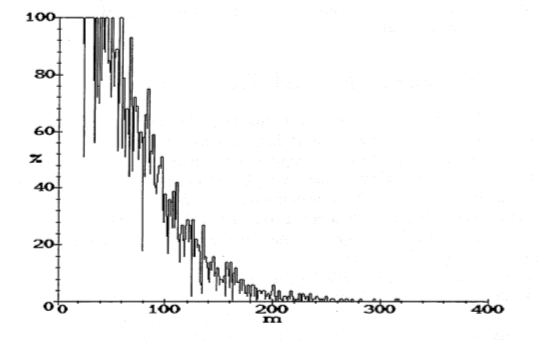
\includegraphics[width=4.16667in,height=3.125in]{Homework 5 Trial and Error 3b646dc8160042df9d000a4baa7eeb4e/Untitled 2.png}
\caption{Hình 1.}
\end{figure}

\textbf{Theorem 2.1}. For all even \(n \ge 6\) there exists a structured
knight's tour on an \(n \times n\) and an \(n \times (n + 2)\) board.
Such a tour can be constructed in time \(O(n^2)\).

Định lý 2.1 khẳng định sẽ luôn tồn tại đường đi cho con mã trong bàn cờ
chẵn với kích cỡ \(N\ge 6\), có thể được dựng trong \(O(N^2)\).

Để thực hiện, ta sẽ tách bàn cờ lớn về những bàn cờ nhỏ hơn, cho đến khi
về trạng thái cơ sở: bàn cờ có kết quả được tính từ trước. Đó là trạng
thái \(8\times 8\). Ta cũng sẽ chỉ quan tâm tới các bàn cờ là bội số của
8.

\begin{figure}
\centering
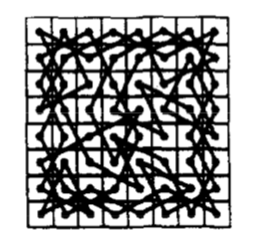
\includegraphics[width=3.125in,height=3.125in]{Homework 5 Trial and Error 3b646dc8160042df9d000a4baa7eeb4e/Untitled 3.png}
\caption{Hình 2.}
\end{figure}

Như đã nói ở trên, khi có đáp án cho trạng thái cơ sở, ta có thể giải
được với \(N = 8k\), \(k\in \mathbb{N}\) . Bằng cách chia nhỏ thành 4
bàn cờ, và đệ quy cho đến khi \(N=8\).

Không mất tính tổng quát, xét vị trí xuất phát ở góc dưới cùng bên trái
(phần D của hình 3(b)). Một khi nước đi chạm rìa trên cùng, thay vì đi
tiếp đến đỉnh D (vẫn ở hình 3(b)) và hoàn thành nước đi, ta đi tiếp sang
đỉnh E (hình 3(c)) và xử lý ở phần bàn ở góc trên trái. Cứ thế từ E sang
F, rồi F sang G\ldots{} Và hoàn thành chuyến đi.

Đây là hình ảnh minh hoạ cho phương pháp này

\begin{figure}
\centering
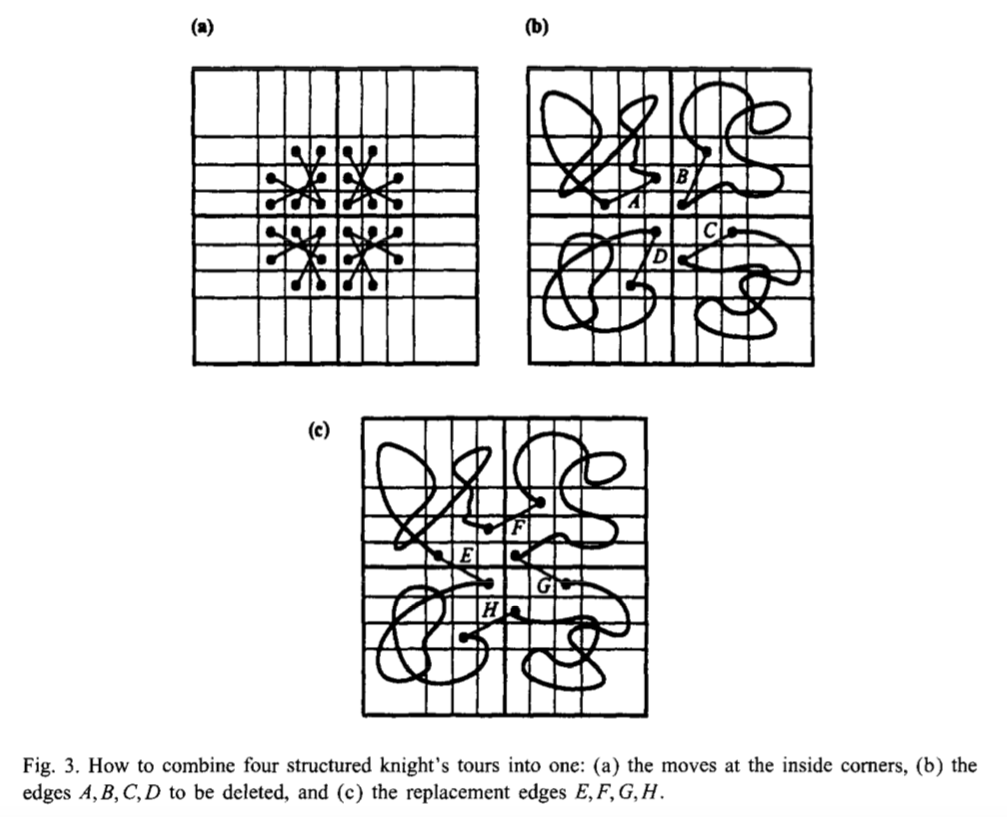
\includegraphics{Homework 5 Trial and Error 3b646dc8160042df9d000a4baa7eeb4e/Untitled 4.png}
\caption{Hình 3.}
\end{figure}

Lưu ý rằng mỗi khi chuyến đi bị đóng lại như trường hợp cơ sở. Tính đóng
của bàn cờ cho phép chúng ta di chuyển sang các góc khác cho đến khi hết
bàn.

Phần code ở trong file đính kèm bài, ở đây sẽ đưa ra các output của
chương trình:

\begin{Shaded}
\begin{Highlighting}[]
\NormalTok{n }\OperatorTok{=} \DecValTok{8}
\NormalTok{board }\OperatorTok{=}\NormalTok{ Chessboard(n,n)}

\BuiltInTok{print}\NormalTok{(board.GetRows())}
\BuiltInTok{print}\NormalTok{(board.GetColumns())}

\BuiltInTok{print}\NormalTok{(}\StringTok{"Building knight path list..."}\NormalTok{)}
\NormalTok{board.FindPathList()}
\BuiltInTok{print}\NormalTok{(}\StringTok{"Building knight tour..."}\NormalTok{)}
\BuiltInTok{print}\NormalTok{()}
\NormalTok{board.FindTour()}
\NormalTok{board.PrintTour()}

\NormalTok{n }\OperatorTok{=} \DecValTok{128}
\NormalTok{board }\OperatorTok{=}\NormalTok{ Chessboard(n,n)}

\BuiltInTok{print}\NormalTok{(}\StringTok{"Building knight path list..."}\NormalTok{)}
\NormalTok{board.FindPathList()}
\BuiltInTok{print}\NormalTok{(}\StringTok{"Building knight tour..."}\NormalTok{)}
\BuiltInTok{print}\NormalTok{()}
\NormalTok{board.FindTour()}
\NormalTok{board.PrintTour()}

\BuiltInTok{print}\NormalTok{(}\StringTok{"Path length:"}\NormalTok{, }\BuiltInTok{len}\NormalTok{(board.GetPathList()))}
\BuiltInTok{print}\NormalTok{(}\StringTok{"Tot. squares:"}\NormalTok{, board.GetColumns() }\OperatorTok{*}\NormalTok{ board.GetRows())}

\NormalTok{board.CheckTour()}
\end{Highlighting}
\end{Shaded}

Output

\begin{Shaded}
\begin{Highlighting}[]
\KeywordTok{(}\ExtensionTok{base}\KeywordTok{)} \ExtensionTok{[10:27:19]}\NormalTok{ [\textasciitilde{}/Documents/mycodes] ❱❱❱ /opt/homebrew/bin/python3 /Users/delus/Documents/mycodes/Classes/Algorithm\_Design\_and\_Analysis/week5/knight\_tour\_d\_a\_c.py}
\ExtensionTok{8}
\ExtensionTok{8}
\ExtensionTok{Building}\NormalTok{ knight path list...}
\ExtensionTok{Building}\NormalTok{ knight tour...}

\ExtensionTok{[[26}\NormalTok{  7 42 11 28 31 56 13]}
 \ExtensionTok{[43}\NormalTok{ 10 27 32 55 12 17 30]}
 \BuiltInTok{[}\NormalTok{ 6 25  8 }\ErrorTok{41} \ExtensionTok{52}\NormalTok{ 29 14 57]}
 \BuiltInTok{[}\NormalTok{ 9 44 33 }\ErrorTok{54} \ExtensionTok{35}\NormalTok{ 16 51 18]}
 \ExtensionTok{[24}\NormalTok{  5 36 47 40 53 58 15]}
 \ExtensionTok{[37}\NormalTok{  2 45 34 61 48 19 50]}
 \BuiltInTok{[}\NormalTok{ 4 23 64 }\ErrorTok{39} \ExtensionTok{46}\NormalTok{ 21 62 59]}
 \BuiltInTok{[}\NormalTok{ 1 38  3 }\ErrorTok{22} \ExtensionTok{63}\NormalTok{ 60 49 20]]}
\ExtensionTok{Building}\NormalTok{ knight path list...}
\ExtensionTok{Building}\NormalTok{ knight tour...}

\KeywordTok{[[}\NormalTok{ 3954  3973  3938 }\ErrorTok{...}  \ExtensionTok{7891}\NormalTok{  7916  7873]}
 \BuiltInTok{[}\NormalTok{ 3937  3970  3953 }\ErrorTok{...}  \ExtensionTok{7872}\NormalTok{  7877  7890]}
 \BuiltInTok{[}\NormalTok{ 3974  3955  3972 }\ErrorTok{...}  \ExtensionTok{7889}\NormalTok{  7874  7917]}
 \ExtensionTok{...}
 \ExtensionTok{[16357}\NormalTok{     2 16365 ... 12118 12153 12120]}
 \BuiltInTok{[}\NormalTok{    4 16343 16384 }\ErrorTok{...} \ExtensionTok{12155}\NormalTok{ 12132 12129]}
 \BuiltInTok{[}\NormalTok{    1 16358     3 }\ErrorTok{...} \ExtensionTok{12130}\NormalTok{ 12119 12154]]}
\ExtensionTok{Path}\NormalTok{ length: 16384}
\ExtensionTok{Tot.}\NormalTok{ squares: 16384}
\ExtensionTok{Complete:}\NormalTok{        True}
\ExtensionTok{Legal:}\NormalTok{           True}
\ExtensionTok{[10:27:20]}\NormalTok{ [cost 0.624s] /opt/homebrew/bin/python3 /Users/delus/Documents/mycodes/Classes/Algorithm\_Design\_and\_Analysis/week5/knight\_tour\_d\_a\_c.py}
\end{Highlighting}
\end{Shaded}

Với \(n = 128\) chỉ mất \(\approx 0.63\)s (code thuật toán
\textbf{Warnsdorff} cũng mất thời gian tương tự nhưng chỉ giải được
\(n=8\)).

\hypertarget{neural-network}{%
\subsection{Neural Network}\label{neural-network}}

Trong quá trình nghiên cứu để làm bài tập, em có đọc qua được những bài
viết về giải bài toán này bằng cách dùng Mạng Neural. Phương pháp này
giúp giải những bài toán có kích thước bàn cờ \(N\) lớn. Ở đây là link
tham khảo chứ không đi sâu vào

\url{https://avinayak.github.io/programming/algorithm/2022/04/01/solving-knights-tour-using-a-neural-network.html}

\end{document}
